\documentclass[12pt]{article}

\usepackage[affil-it]{authblk}
\usepackage[shortlabels]{enumitem}
\usepackage[utf8]{inputenc}
\usepackage{algorithm, algorithmicx, algpseudocode}
\usepackage{amsfonts, amsthm, amsmath, amssymb}
\usepackage{color}
\usepackage{cancel, textcomp}
\usepackage{enumerate}
\usepackage[mathscr]{euscript}
\usepackage{fancyhdr, fancyvrb}
\usepackage{fullpage}
\usepackage[left=0.5in,right=0.5in,headsep=0.5in,headheight=0.5in]{geometry}
\usepackage{graphicx}
\usepackage{hyperref}
\usepackage{latexsym}
\usepackage{mathtools}
\usepackage{minted}
\usepackage{times}
\usepackage{xcolor}
\usepackage{physics}
\usepackage{tikz-cd}
\usepackage[warnunknown, fasterrors, mathletters]{ucs}
\usepackage[nointegrals]{wasysym}

\newcommand{\hw}[2]{
    \noindent
    \begin{center}
        \framebox{
            \vbox{
                \hbox to 7in { {\bf MATH 470: Communications and Cryptography } \hfill  }
                \vspace{2mm}
                \hbox to 7in { {\Large \hfill Homework #1\hfill} }
                \vspace{2mm}
                \hbox to 7in { {\it Due date: #2 \hfill Name: Huy Lai } }
            }
        }
    \end{center}
    \vspace*{4mm}
}

\newcounter{prob}
\setcounter{prob}{0}
\newcounter{subprob}
\setcounter{subprob}{0}

\newcommand{\problem}{\setcounter{subprob}{0}\stepcounter{prob}{\noindent\textbf{Problem \theprob.}}\ }
\newcommand{\subproblem}{\stepcounter{subprob}{\noindent\textbf{Subproblem \thesubprob.}}\ }
\newcommand{\solution}{\noindent\textbf{Solution:}\newline}

\newcommand{\babc}{\begin{enumerate}[a)]}
\newcommand{\eabc}{\end{enumerate}}

\everymath{\displaystyle}

\setlength{\parskip}{.1in}
\setlength{\headheight}{15pt}
\setlength{\topmargin}{0pt}

\fancyhf{}
\pagestyle{fancy}
\lhead{MATH 470: Communications and Cryptography}
\rhead{Texas A\&M University}
\cfoot{\thepage}


\begin{document}
\hw{4}{20 September 2023}

\problem Alice and Bob agree to use the prime $p=1373$ and the base $g=2$ for a Diffie–Hellman key exchange. Alice sends Bob the value $A=974$. Bob asks your assistance, so you tell him to use the secret exponent $b=871$. What value $B$ should Bob send to Alice, and what is their secret shared value? Can you figure out Alice’s secret exponent?

\solution
Bob's sends $B=g^b\mod{p}\equiv805\mod{1375}$ to Alice.\\
Their shared secret is $A^b\mod{p}\equiv397\mod{p}$

\noindent
There is no really easy way to determine Alice’s secret exponent, but with a computer or even a programmable calculator, it does not take long to compute all of the powers of $2\mod{1373}$.

\newpage
\problem Alice and Bob agree to use the prime $p=1373$ and the base $g=2$ for communications using the Elgamal public key cryptosystem.

\subproblem Bob chooses $b=716$ as his private key, so his public key is
\[B\equiv 2^{716}\equiv469\mod{1373}\]
Alice encrypts the message $m=583$ using the random element $k=877$. What is the ciphertext $(c_1,c_2)$ that Alice sends to Bob?

\solution
$c_1=g^k\mod{p}\equiv 719\mod{1373}$\\
$c_2=m\cdot B^k\mod{p}\equiv 623\mod{1373}$\\
$(c_1,c_2)=(719,623)$

\subproblem
Alice decides to choose a new private key $a=299$ with associated public key $A\equiv2^{299}\equiv34\mod{1373}$. Bob encrypts a message using Alice’s public key and sends her the ciphertext $(c_1,c_2)=(661,1325)$. Decrypt the message.

\solution Decrypting the message is as follows
\begin{flalign*}
    m & = \left(c_1^{-1}\right)^{a}c_2\mod{p} & \\
      & = (661^{299})^{-1}\cdot1325\mod{1373} & \\
      & = 645^{-1}\cdot1325\mod{1373}         & \\
      & = 794\cdot1325\mod{1373}              & \\
      & = 332
\end{flalign*}

\newpage
\problem Suppose that Eve is able to solve the Diffie–Hellman problem. More precisely, assume that if Eve is given two powers $g^u$ and $g^v\mod{p}$, then she is able to compute $g^{uv}\mod{p}$. Show that Eve can break the ElGamal PKC.

\solution
In the Engamal PKC, Eve knows Alice's public key $A\equiv g^u\mod{p}$ and Eve knows the ciphertext consiting of two integers $c_1\equiv g^v\mod{p}$ and $c_2\equiv m\cdot A^v\mod{p}$.\\
Given Eve knows $g^u$ and $g^v\mod{p}$, she can compute $g^{uv}\mod{p}$.\\
With this, she can recover the encrypted message by computing $\left(g^{uv}\right)^{-1}\cdot c_2\equiv m\mod{p}$

\problem Use Shanks’s babystep–giantstep method to solve the following discrete logarithm problem.
\[11^x=21 \text{ in } \mathbb{F}_{71}\]

\solution
Since $\gcd(11,71)=1$, we can apply Fermat's Little Theorem to it to calculate the order.
The number $11$ has order $70$ in $\mathbb{F}_{71}$.\\
Set $n=\left\lceil\sqrt{70}\right\rceil=9$.\\
By Fermat's Little Theorem we can calculate $g^{-n}\equiv g^{n\cdot(p-2)}\mod{p}=7$

\noindent
\begin{tabular}{|c|c|c|}
    \hline
    $i$ & $g^i\mod{71}$ & $hg^{-in}\mod{71}$ \\
    \hline
    $0$ & $1$           & $21$               \\
    $1$ & $11$          & $5$                \\
    $2$ & $50$          & $35$               \\
    $3$ & $53$          & $32$               \\
    $4$ & $15$          & $11$               \\
    $5$ & $23$          & $6$                \\
    $6$ & $40$          & $42$               \\
    $7$ & $14$          & $10$               \\
    $8$ & $12$          & $70$               \\
    $9$ & $61$          & $64$               \\
    \hline
\end{tabular}

\noindent
$i=1,j=4$\\
Therefore, the solution is $x=4\cdot9 + 1= 37$

\newpage
\problem Let $p\geq3$ be a prime and suppose that the congruence $X^2\equiv b\mod{p}$ has a solution.
Prove that the congruence $X^2\equiv b\mod{p^2}$ also has a solution.

\solution To prove that if the congruence $X^2 \equiv b \mod{p}$ has a solution, then the congruence $X^2 \equiv b \mod{p^2}$ also has a solution, we can use the Chinese Remainder Theorem (CRT) and a bit of algebraic manipulation.

\begin{proof}
    Let $x_1$ be a solution to $X^2 \equiv b \mod{p}$.\\
    Assume that $X = x_1 + kp,k\in\mathbb{Z}$

    \noindent
    Now, we'll square $X$ and see what we get:
    \begin{flalign*}
        X^2 & = (x_1 + kp)^2            &   \\
            & = x_1^2 + 2kpx_1 + k^2p^2 & .
    \end{flalign*}

    \noindent
    Now, let's consider the congruence $X^2 \equiv b \mod{p^2}$. Substituting our expression for $X^2$, we have:
    \[x_1^2 + 2kpx_1 + k^2p^2 \equiv b \mod{p^2}\]

    \noindent
    Now, notice that $x_1^2 \equiv b \mod{p}$ by our assumption. Additionally, $k^2p^2$ is a multiple of $p^2$. So, we can simplify the congruence to:
    \[b+2kpx_1\equiv b\mod{p^2}\]
    By proposition, this implies that $p^2\mid (2kpx_1+b-b)\rightarrow p^2\mid 2kpx_1$.

    \noindent
    This shows that for $k\in\mathbb{Z}$, $X=x_1+kp$ satisfies the congruence $X^2\equiv b \mod{p^2}$. Therefore, we have found a solution to $X^2 \equiv b \mod{p^2}$, given that a solution exists for $X^2 \equiv b \mod{p}$.
\end{proof}

\newpage
\problem Let $p$ be a large prime and let $g$ be a primitive root $\mod{p}$. Suppose $p$ and $g$ are publicly known to everybody in a network. Alice chooses a secret integer $a$ and publishes $A=g^a\mod{p}$ as her public key by broadcasting it over the network. Bob wants to send Alice a message $m$ using Elgamal
encryption.\\
Suppose however that an active adversary Eve has the ability to intercept and modify messages sent over the network (including Alice’s broadcasting of her public key) without being detected. Show how Eve can perform a Man-In-The-Middle attack.

\solution
Alice first publishes $A=g^a\mod{p}$ as her public key.\\
Eve intercepts this and chooses a secret integer $e$ and publishes $E=g^e\mod{p}$ as Alice's fake key.\\
Using this, Bob computes $c_1=g^b\mod{p}$ and $c_2=m\cdot E^b\mod{p}$ sends this message to Eve.\\
Eve than decrepit the message received from Bob, modifies it to her liking and then sends the new message $c_{1e},c_{2e}$ to Alice.\\
Alice then computes $(c_{1e}^a)^{-1}\cdot c_{2e}\equiv m_e\mod{p}$.\\
This completes the Man-In-The-Middle attack.

\newpage
\problem You may assume that $p=123456789001907$ is prime and that $2$ is a primitive root modulo $p$. Find an integer $x$ such that $2^x\equiv3\mod{p}$.

\solution
\setminted{fontsize=\small,baselinestretch=1}
\inputminted{py}{lsbs.py}

\begin{figure}[!ht]
    \centering
    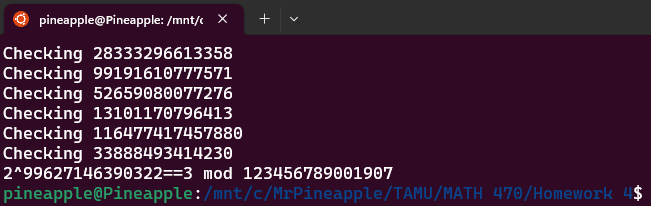
\includegraphics[width=\textwidth]{Question 7.png}
    \caption{Output}
\end{figure}

\end{document}
